The main component of our system is the "Core Component" which is responsible for estimating the weight of a cattle given an RGB image along with a per-pixel depth map. So, most of the time was spent in in the development of this component. The experiments which we carried out throughout the span of this project can be divided into the following two main categories.
\begin{enumerate}
\item Deep learning Models 
\item Camera and Depth Related Experiments 
\end{enumerate}
\subsection{Deep Learning Models}
Almost \(75\%\) of the time was dedicated to collect data whose description is in 3.5.5 Dataset and Augmentation section, to do experiments, and to come up with a better model. The biggest challenge for this part was the availability of dataset and also weight of the cattle. All dataset, which is used throughout this project, is collected by our team. 
\\

\subsubsection{Experiments on Dataset V1 for Localization}

On dataset V1, we tried to solve our problem as a localization problem through transfer learning. In localization problem we assume that there is only one object in an image which we are trying to detect. This fact give us an advantage that we know exactly how many bounding boxes we have to predict. In this experiment Pre-trained networks VGG16 and Resnet were used as base networks. At the end of these networks we attached our own fully connected network for regression on the features extracted by the base networks. 

Initially, we trained only fully connected layers for two bounding boxes. Then we trained only fully connected layers for one bounding box. We then unfreeze some convolution layers and train them for both two bounding boxes and one bounding box. Global Average Pooling was used for Localization. But we were unable to get the satisfactory results. Our min loss was 4.68 on mean absolute error. 

\begin{figure}[h]
\centering
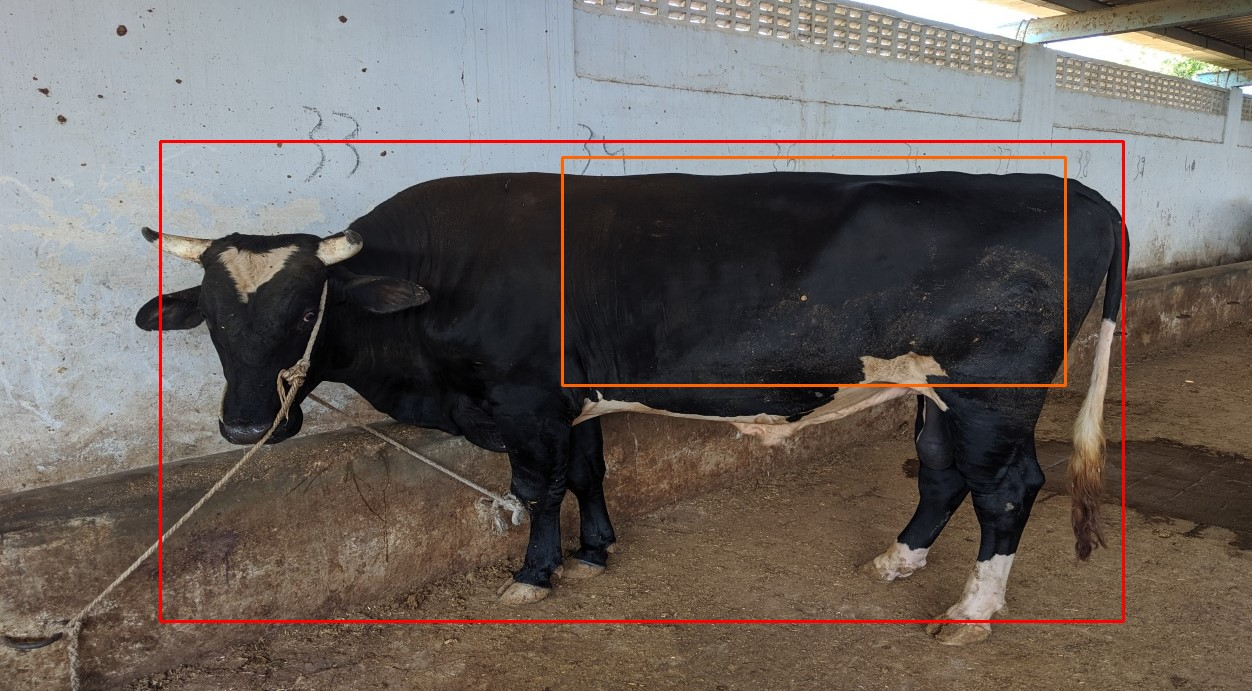
\includegraphics[scale=0.3]{v1-loc.jpg}
\caption{Output of Models for Object Localization trained on V1}
\end{figure}


\begin{figure}[h]
\centering
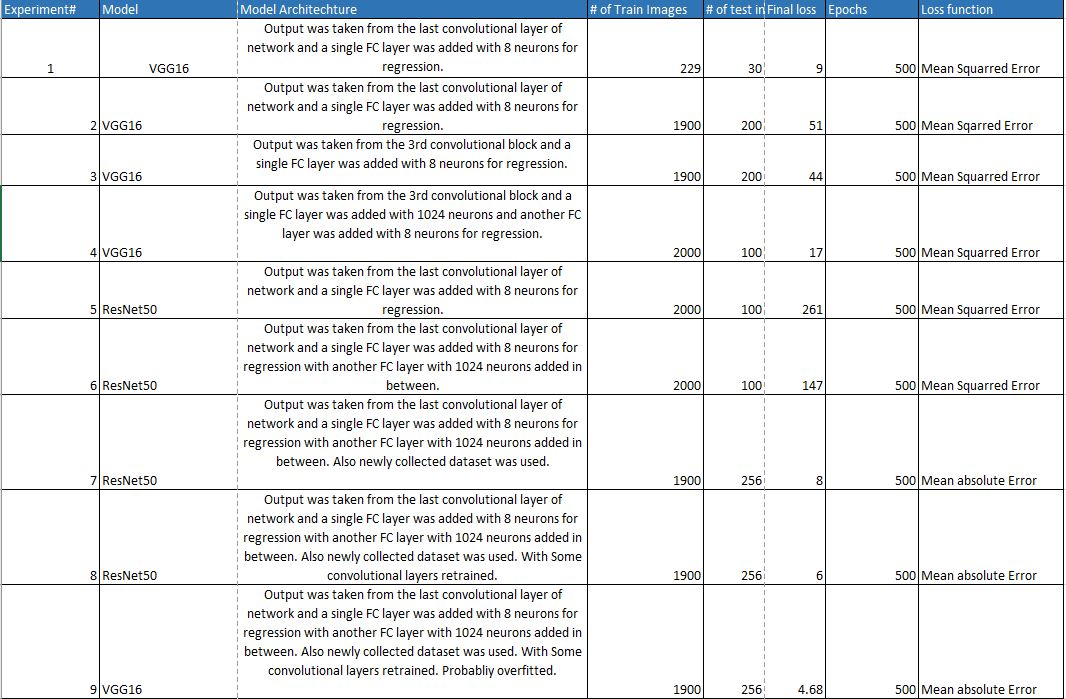
\includegraphics[scale=0.5]{Capture.JPG}
\caption{Results of Models for Object Localization trained on V1}
\end{figure}
\pagebreak



\subsubsection{Experiments on Dataset V2 for Localization}
In this experiment, cattle images were cropped and we tried to predict inner bounding boxes. We assumed that it will learn better features due to the lack of background. However, this did not produce the results we were looking for

The problem we observed in both of the experiments was the over fitting of train data. They seemed to perform good on train data while it performed worse on test data. But in order to make our solution work we needed very tight bounding box. After a lot of effort we then trained Yolo and Mask RCNN. 

\subsubsection{YOLO}
After experimenting with object localization and not getting satisfactory results we turned towards YOLO object detector. YOLO stands for You Only Look Once. The advantages of using YOLO are numerous and one of them is speed, YOLO is the fastest deep learning based object detector which offers reasonable accuracy.
We trained YOLO on Dataset V2 containing 1200 images. After 100 epochs we got loss of 11.54 units on YOLO custom loss function.
On the test set we acheived an average IoU of \(80\%\).
The bounding box detected by YOLO trained on dataset V2 is shown below.\\
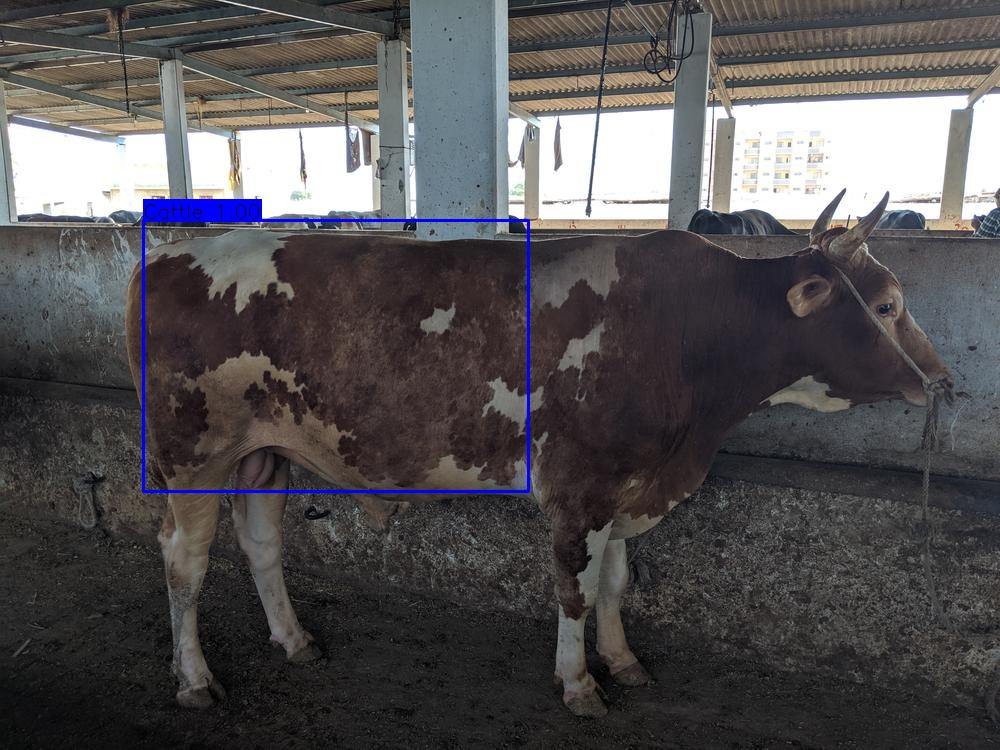
\includegraphics[scale = 0.2]{images/result.jpg}

The results from YOLO may look reasonable but they could be made better with little adjustment. Or we can collect a bigger dataset and train YOLO on it better performance in terms of detection accuracy. In an ideal case there should not be a single pixel on the box that is outside cattle body.

\subsubsection{Mask R-CNN}

In our quest for a perfect weight estimater we also explored Mask R-CNN to get a better more robust system. The idea was to segment out the cattle from the RGB image. Then superimpose the cattle mask on the depth channel. Essentially, the extracting all the depths the lies on the cattle. We then input the depth values to an Artificial Neural Network (ANN) and frame the problem as regression problem. The problem with this approach is that it needs weight labels for each cattle in the dataset, which is not available. Nevertheless we went on to explore this approach as weight labels can be collected later.\\

We trained a Mask-RCNN on Dataset V2 and got the following results.\\
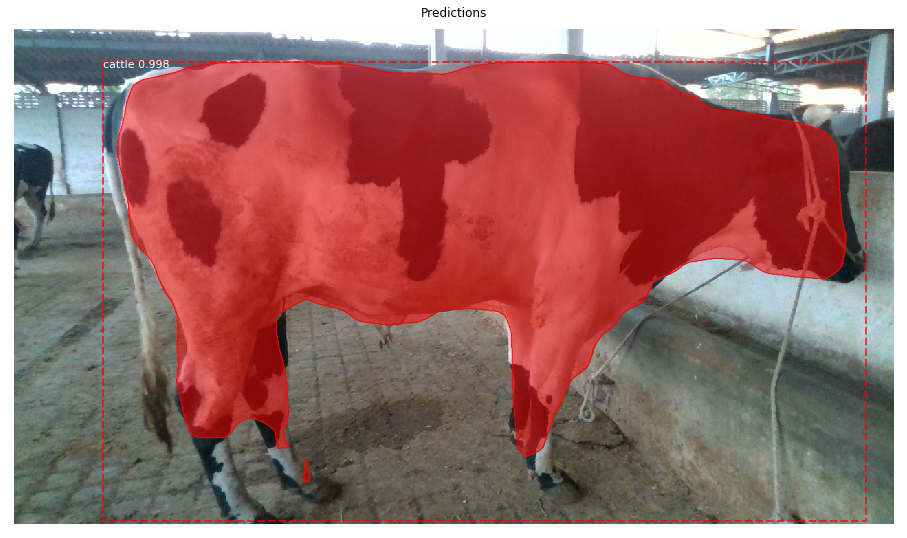
\includegraphics[scale=0.3]{images/1122.png}\\


But we can not proceed any further with this approach to make an actual weight estimator as we dont have weight labels of each cattle. But what we can do is prove that the ANN which we are going to train once we get the weight labels will work, by calculating the proxy Factor in the next sub heading.

\subsubsection{Factor}


\subsection{Camera and Depth Related Experiments}
The purpose of our deep learning models to get the rectangle so that we can take out the pixels' vector which lies on the heart girth of the cattle once we have this vector we have to get the real world measurement of the heat girth of the cattle. 


\subsubsection{Curve Length Estimation:}

In the above mentioned approaches the final result we get is a bounding box encapsulating the information of body length in the diagonal and heart girth measurements in height of the box. Since these values are just only represented by two pixel coordinates top-left and bottom right. As mentioned earlier to get the measurements accurate we have to incorporate the depth information. Since we have depth map and RGB image of same dimensions and from same camera we can safely map this bounding box to depth image as well. 

Once we have a this image box on depth image we will extract out the vector of pixels from the heart girth line of the bounding box and diagonal vector from pixels starting from bottom left and the top right  point in this image.
Once we have these two vectors we can convert it into real world measurements using the procedure defined below.   
For the simplicity forget the consider that we have a formula which converts  given number of pixels into meters and also take a distance from camera to take care of the scaling, because otherwise far objects appear small in image. now given this formula consider the abdomen of the cattle. It is mostly symmetric from both sides. If we take the measurements of a heart girth and body length curves on the surface of the abdomen, which is like a semi-ellipse from one side, will have huge factor in measurements. So to preserve this information we will use the mathematical approach, discussed in Appendix A, to get the length of heart girth circumference and body length more accurately. 






 

 
